\documentclass[]{article}

\usepackage{tabu}
\usepackage{amsfonts}
\usepackage{amsmath}
\usepackage{graphicx}

\setlength{\tabcolsep}{12pt}
\renewcommand{\arraystretch}{2}

%opening
\title{CSE 306\_Assignment1 \\
4-Bit Arithmetic and Logic Unit}
\author{ \\ Student ID : 1505097-1505102}





\begin{document}
\maketitle

\vspace{5cm}

\begin{figure}[h!]
    \centering
    
\includegraphics[width = 0.3\textwidth]{logo.png}
    \label{fig:bl}
\end{figure}
\begin{center}
   \Large{ Department of Computer Science and Engineering
 \\ Bangladesh University of Engineering and Technology
 \\ (BUET) \\
Dhaka 1000 \\}

\end{center}



\newpage
	%--------------------------------------------------------arithmetic
	\section{Design of Arithmetic Unit}
	
	\textbf{Truth Table : Arithmetic Operations}
	\begin{center}
		\begin{tabular}{ |c|c|c|c|c|c|c| } 
			\hline
			$CS_2$ & $CS_1$ & $CS_0(C_{in})$ & $X_i$ & $Y_i$ & $F$ & Arithmetic Operation  \\
			\hline
			
			\hline
			0 & 0 & 0 & $A_i$ & $\overline{B_i}$ & $A-B-1$ & Subtract with borrow \\
			\hline

			\hline
			0 & 0 & 1 & $A_i$ &$\overline{B_i}$ & $A-B$ & Subtract \\
			\hline
			
			\hline
			0 & 1 & 0 & $A_i$ & $1$ & $A-1$ & Decrement A \\
			\hline
			
			\hline
			0 & 1 & 1 & $A_i$ & $1$ & $A$ & Transfer A \\
			\hline
			
		\end{tabular}
	\end{center}
	\noindent\textit{Subtract with borrow :}\newline
	$=A-B-1$ \newline
	$=(A+\overline{B}+1)-1$ \newline
	$=A+\overline{B}$ \newline
	$=A+(2^n-1-B)$\newline
	$=2^n+(A-B-1)$\newline

	\noindent\textit{Subtract : } \newline
	$=A-B$ \newline
	$=A+\overline{B}+1$ \newline
	$=A+(2^n-1-B)+1$\newline
	$=2^n+(A-B)$\newline

	\noindent\textit{Decrement A :}\newline
	$=A-1$ \newline
	$=A+2^n-1 $ \newline
	$=2^n+(A-1)$ \newline

	\noindent\textit{Transfer A :}\newline
	$=A$ \newline
	$=A+2^n-1+1 $ \newline
	$=2^n+A$
	\newline

	\noindent So we have, \newline\\
	$X_i=A_i$\\\\
	$Y_i=\overline{CS_1}.\overline{B_i}+CS_1 = \overline{(CS_1+B_i)}+CS_1$
	\begin{figure}[h!]
		\centering
		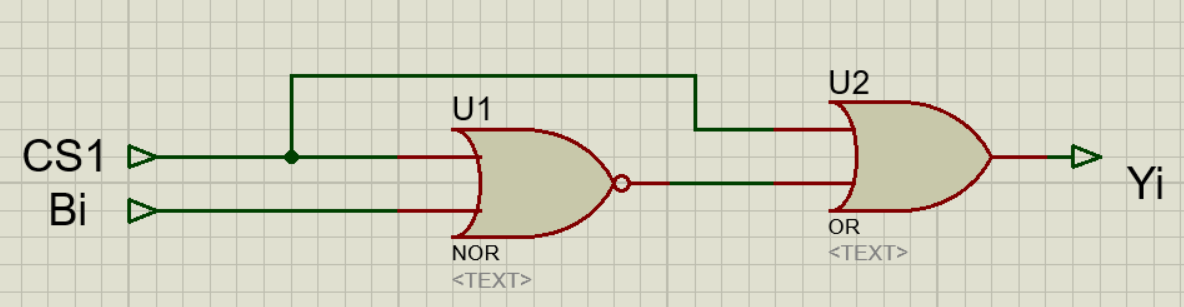
\includegraphics[width = 0.5\textwidth]{Yi.PNG}
		\caption{Design of Yi}
		\label{fig:ckt1}
		
	\end{figure}
	%--------------------------------------------------------arithmetic
	
	%--------------------------------------------------------logic
	\section{Design of Logic Unit}
	\textbf{Truth Table : Logical Operations}
		\begin{center}
		\begin{tabular}{ |c|c|c|c|c|c|c| } 
			\hline
			$CS_2$ & $CS_1$ & $CS_0(c_{in})$ & $X_i$ & $Y_i$ & $F_i=X_i \oplus Y_i$ & Operation \\
			\hline
			
			\hline
			1 & 0 & 0 & $A_i+\overline{B_i}$ & $B_i$ & $A_i.B_i$ & AND \\
			\hline
			
			\hline
			1 & 0 & 1 & $A_i+\overline{B_i}$ & $B_i$ & $A_i.B_i$ & AND \\
			\hline
			
			\hline
			1 & 1 & 0 & $\overline{A_i}$ & $1$ & $\overline{A_i}$ & Complement A \\
			\hline
			
			\hline
			1 & 1 & 1 & $\overline{A_i}$ & $1$ & $\overline{A_i}$ & Complement A\\
			\hline
		\end{tabular}
	\end{center}

	\noindent\textbf{Explanation:}
	We can't modify $Y_i$ because that would change the arithmetic operations
	and neither can omit $A_i$ in any input, So we change $X_i$.\newline
	Let,
    \\$X_i=A_i+K_i$ \newline
    
    \noindent$F_i=X_i \oplus Y_i$\newline
	$F_i=(A_i \oplus K_i) \oplus \overline{B_i}$\newline
	$F_i=(A_i \oplus K_i)B_i + \overline{(A_i \oplus K_i)} .\overline{B_i}$\newline
	$F_i=A_iB_i + K_iB_i + \overline{A_i}.\overline{K_i}.\overline{B_i}$ \newline 
	
	\noindent Here the desired operation is $A_iB_i$. So putting $K_i=\overline{B_i}$ \newline
	$F_i=A_iB_i$\newline
	
	\noindent$F_i=X_i \oplus Y_i$ \newline
	$F_i=X_i \oplus 1$ \newline
	$F_i=\overline{X_i}$ \newline
	$F_i=\overline{A_i+K_i}$\newline
	
	\noindent Here the desired output is $\overline{A_i}$. So putting $K_i=0$ \newline
	$F_i=\overline{A_i}$\newline
	
	\noindent So we need $K_i=\overline{B_i}$ when we will do AND operation and $K_i=0$ for NOT operation.
	
	\noindent We get, \newline\\
	$X_i=A_i+CS_2.\overline{CS_1}.\overline{B_i}=A_i+CS_2\overline{(CS_1+B_i)} $\newline
	
	\begin{figure}[h!]
		\centering
		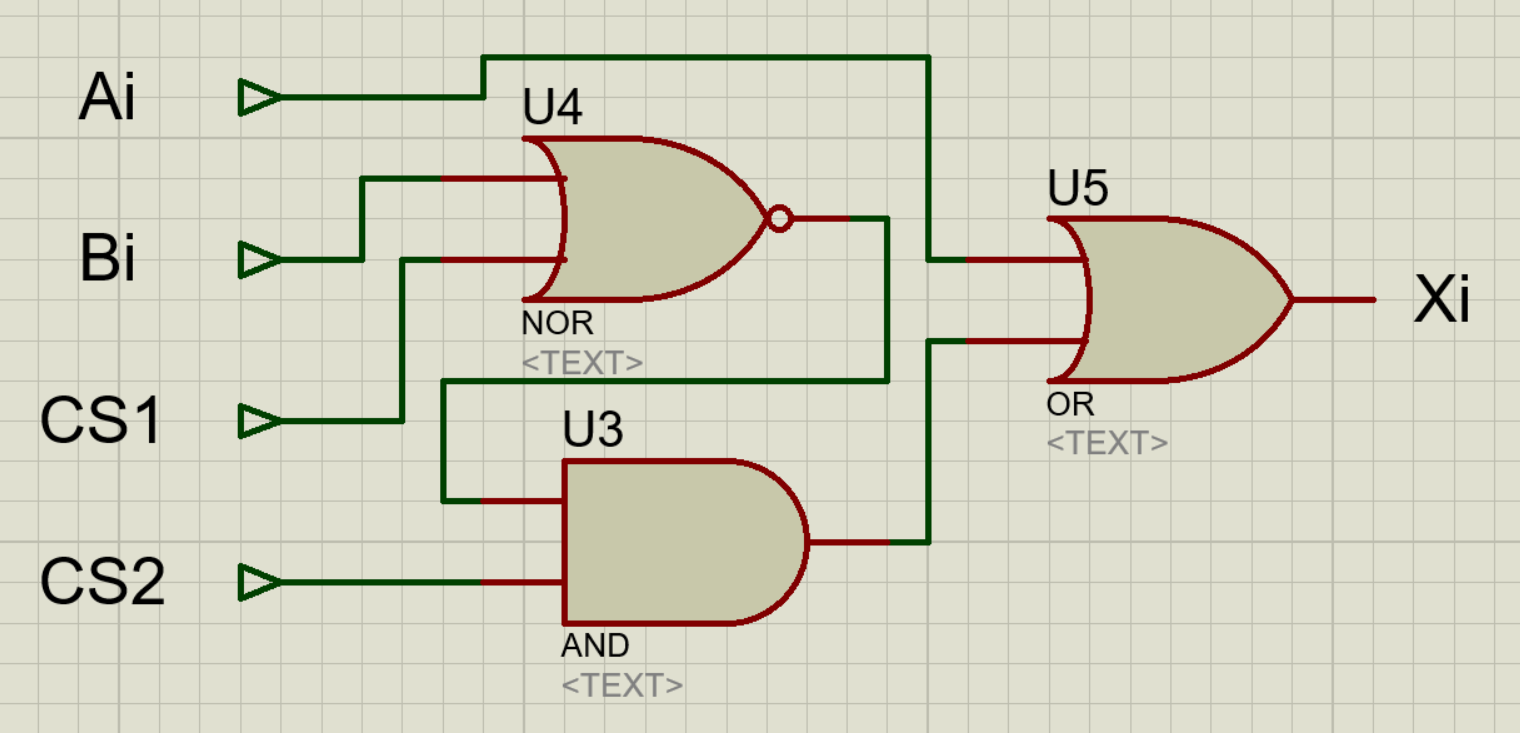
\includegraphics[width = 0.5\textwidth]{Xi.PNG}
		\caption{Design of $X_i$ \newline
		}
		\label{fig:ckt2}
		
	\end{figure}
    \noindent So finally we have,\\\\
	$X_i=A_i+CS_2\overline{(CS_1+B_i)}$
	\newline
	\newline
    $Y_i = \overline{(CS_1+B_i)}+CS_1$
    
	
	
	%--------------------------------------------------------logic	
\end{document}